\documentclass[tikz,border=0pt]{standalone}
\usepackage[utf8]{inputenc}
\usepackage[T1]{fontenc}
\usepackage{lmodern}
\usepackage{amsmath,amssymb}
\usetikzlibrary{arrows.meta,positioning,fit,calc,backgrounds,shapes.geometric,decorations.pathreplacing}
\definecolor{navy}{HTML}{163A5F}
\definecolor{blue}{HTML}{2C6EAF}
\definecolor{lightblue}{HTML}{EAF2F8}
\definecolor{midblue}{HTML}{CFE1F2}
\definecolor{graytext}{HTML}{4A5560}
\definecolor{lightgray}{HTML}{F4F6F8}
\definecolor{green}{HTML}{3C8D73}
\definecolor{lightgreen}{HTML}{E8F5EF}
\definecolor{red}{HTML}{B24A4A}
\definecolor{lightred}{HTML}{FBEDEE}
\tikzset{
  title/.style={font=\sffamily\bfseries\fontsize{18}{20}\selectfont,text=navy,anchor=west},
  subtitle/.style={font=\sffamily\bfseries\fontsize{11}{13}\selectfont,text=navy},
  body/.style={font=\sffamily\fontsize{9.2}{11}\selectfont,text=graytext,align=left},
  small/.style={font=\sffamily\fontsize{8}{9.4}\selectfont,text=graytext,align=left},
  tinylabel/.style={font=\sffamily\fontsize{7.2}{8.4}\selectfont,text=graytext},
  panel/.style={rounded corners=3pt,draw=midblue,fill=white,line width=0.6pt},
  box/.style={rounded corners=2pt,draw=midblue,fill=lightblue,line width=0.6pt},
  worker/.style={rounded corners=2pt,draw=blue,dashed,line width=0.7pt,fill=white},
  task/.style={rounded corners=2pt,draw=blue,fill=lightblue,minimum width=0.85cm,minimum height=0.55cm,font=\sffamily\bfseries\small,text=navy},
  file/.style={draw=blue,fill=white,minimum width=0.55cm,minimum height=0.42cm,font=\sffamily\small,text=navy},
  arr/.style={-{Stealth[length=2.4mm,width=1.8mm]},draw=blue,line width=0.9pt},
  arrthin/.style={-{Stealth[length=2mm,width=1.5mm]},draw=blue,line width=0.7pt},
  arrred/.style={-{Stealth[length=2mm,width=1.5mm]},draw=red,dashed,line width=0.8pt},
  arrgreen/.style={-{Stealth[length=2mm,width=1.5mm]},draw=green,dotted,line width=1pt}
}
\begin{document}

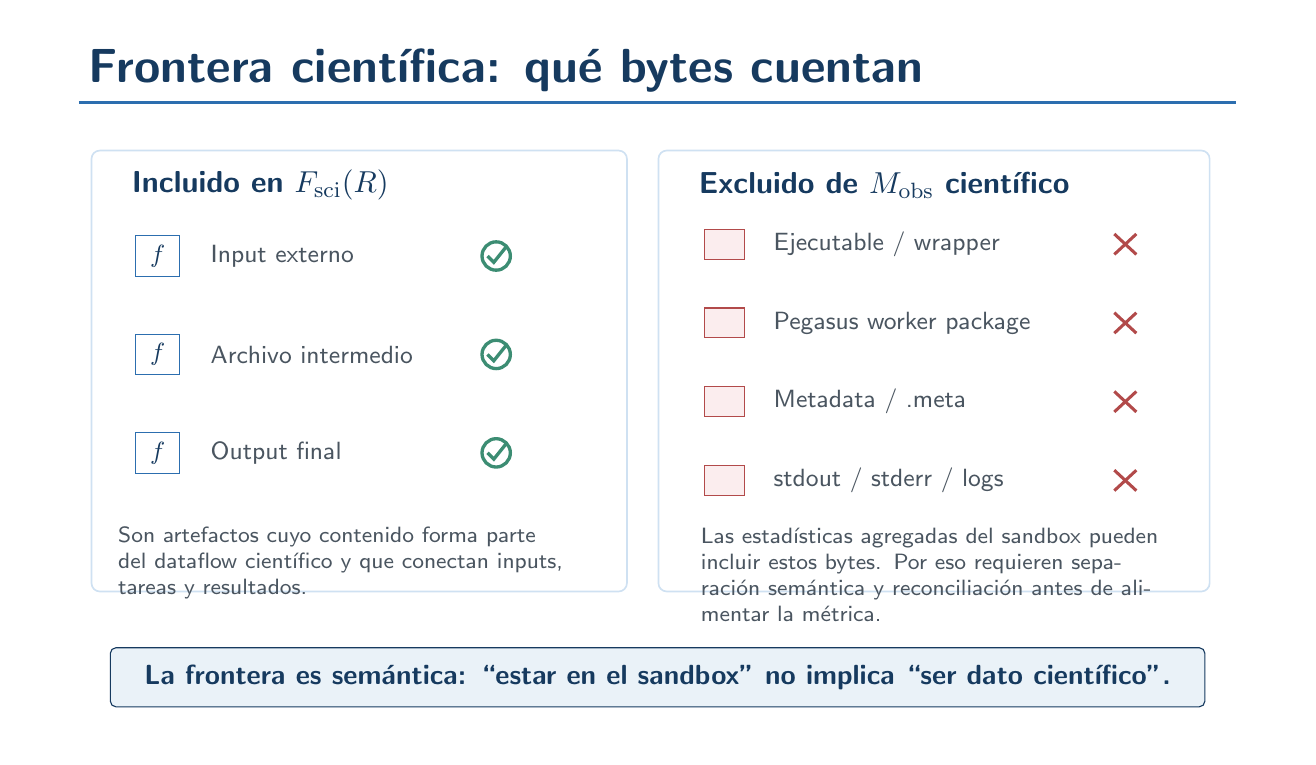
\begin{tikzpicture}[x=1cm,y=1cm]
\path[use as bounding box] (0,0) rectangle (16,9);
\node[title] at (0.65,8.45) {Frontera científica: qué bytes cuentan};
\draw[blue,line width=1pt] (0.65,8.05)--(15.35,8.05);
\node[panel,minimum width=6.8cm,minimum height=5.6cm,anchor=north west] at (0.8,7.45) {};
\node[subtitle,anchor=west] at (1.2,7.0) {Incluido en $F_{\mathrm{sci}}(R)$};
\foreach \y/\lab in {6.1/{Input externo},4.85/{Archivo intermedio},3.6/{Output final}}{
 \node[file] at (1.65,\y) {$f$};
 \node[body,anchor=west] at (2.2,\y) {\lab};
 \draw[green,line width=1.2pt] (5.95,\y) circle (0.18); \draw[green,line width=1.2pt] (5.84,\y)--(5.92,\y-0.08)--(6.08,\y+0.12);
}
\node[small,text width=5.7cm] at (4.0,2.2) {Son artefactos cuyo contenido forma parte del dataflow científico y que conectan inputs, tareas y resultados.};

\node[panel,minimum width=7.0cm,minimum height=5.6cm,anchor=north west] at (8.0,7.45) {};
\node[subtitle,anchor=west] at (8.4,7.0) {Excluido de $M_{\mathrm{obs}}$ científico};
\foreach \y/\lab in {6.25/{Ejecutable / wrapper},5.25/{Pegasus worker package},4.25/{Metadata / .meta},3.25/{stdout / stderr / logs}}{
 \node[draw=red,fill=lightred,minimum width=0.5cm,minimum height=0.38cm] at (8.85,\y) {};
 \node[body,anchor=west] at (9.35,\y) {\lab};
 \draw[red,line width=1.1pt] (13.8,\y-0.13)--(14.08,\y+0.13); \draw[red,line width=1.1pt] (13.8,\y+0.13)--(14.08,\y-0.13);
}
\node[small,text width=5.9cm] at (11.5,2.05) {Las estadísticas agregadas del sandbox pueden incluir estos bytes. Por eso requieren separación semántica y reconciliación antes de alimentar la métrica.};
\node[rounded corners=2pt,draw=navy,fill=lightblue,minimum width=13.9cm,minimum height=0.75cm,font=\sffamily\bfseries,text=navy] at (8,0.75) {La frontera es semántica: “estar en el sandbox” no implica “ser dato científico”.};
\end{tikzpicture}
\end{document}
